% !TeX encoding=utf8
% !TeX spellcheck = de-DE
\section{Theoretische Lösungsansätze}
\subsection[Die reduzierte Druckansicht]{Ansatz 1: Druckansicht}% \addcontentsline{toc}{subsection}{Ansatz 1: Druckansicht} % Add to table of contents without enumerating
\label{extractor:ansatz:subsec1}
Der erste Ansatz, den wir in Betracht gezogen haben, um den Inhalt eines Artikels zu extrahieren war die \quote{Druckansicht} der Seite zu verwenden. Hiermit ist diejenige Version des Artikels gemeint, welche erzeugt werden würde, wenn man mit einem Browser die Seite auf Papier ausdruckt. Wie uns aufgefallen ist, besitzen einige Seiten eine Druckansicht, die sich von der dargestellten Version unterscheiden, oft indem Elemente wie Navigation, Bilder und Werbung entfernt sind und fast nur der Inhalt dargestellt wird. Beispielsweise die News – Seite \url{www.heise.de} besitzt für all ihre Artikel eine solche Druckversion. (siehe Abb. \ref{extractor:image:druckansicht})

\begin{figure}[t]
	\centering
	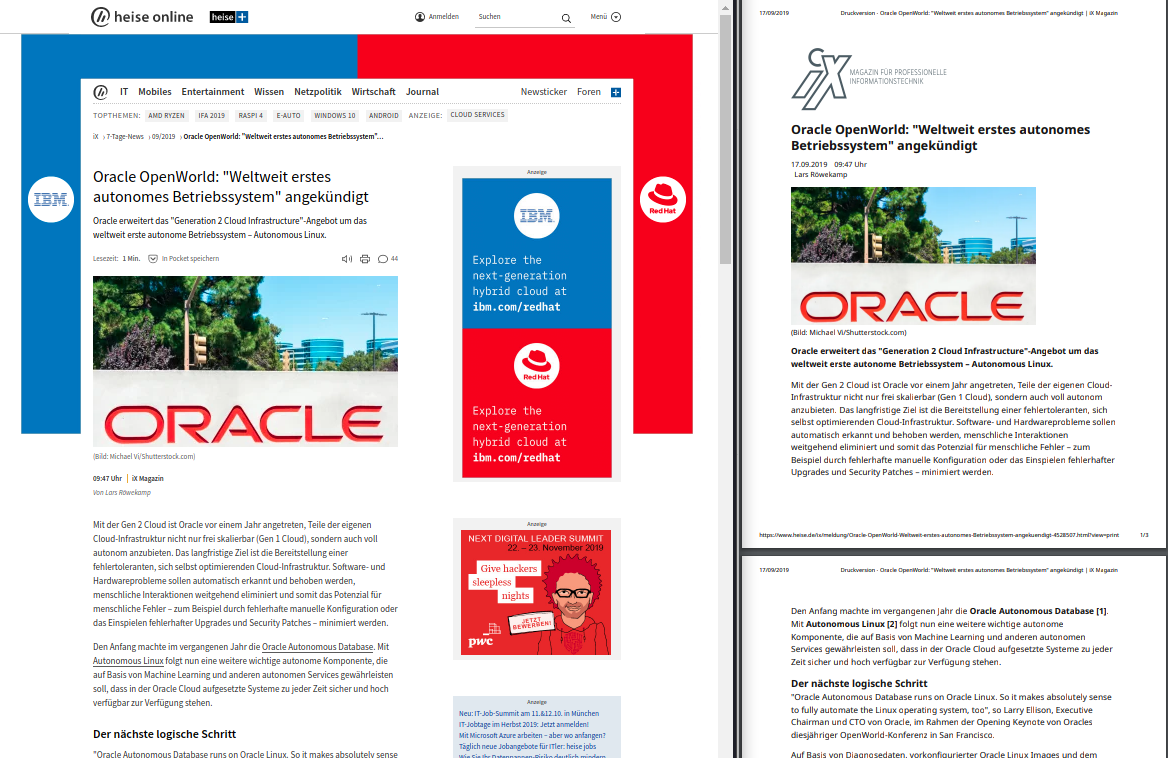
\includegraphics[width=\linewidth]{images/druckansicht.png}
	\caption{Ein Artikel und dessen reduzierte Druckversion}
	\label{extractor:image:druckansicht}
\end{figure}

Man sieht wie die vollständige Website auf der linken Seite Navigationselemente und Werbung, die wir als nicht relevant ansehen enthält. Rechts sind dahingegen nur die relevanten Inhalte zu sehen. Falls wir also in der Lage sind, zu einem solchen Artikel vom Link auf diese Druckansicht zu schließen, könnten wir diese verwenden, um den relevanten Text einer Website zu bestimmen. Um diesen Lösungsansatz zu implementieren muss man mit zwei zentralen Fragen beschäftigen.
\begin{enumerate}
	\item Wie erhält man die Druckansicht des Artikels, falls diese existiert?
	\item Kann man bestimmen ob eine Website überhaupt eine reduzierte Druckansicht hat? 
\end{enumerate}
Ein Werkzeug zur Lösung der ersten Frage sind \quote{headless} Webbrowser. Der Begriff \quote{headless} beschreibt hierbei, dass ein Programm, welches normalerweise mit einer grafischen Benutzeroberfläche ausgeführt wird, komplett ohne diese rein algorithmisch gesteuert wird. Wir werden in Abschnitt \ref{todo} sehen, wie man einen headless Browser verwendet, da wir für das Rendern von Bildern die gleiche Herausforderung haben werden. \\ \\
Aufgrund der zweiten Frage müssen wir leider feststellen, dass dieser Lösungsansatz nicht ausreichend ist. So gibt es keinen uns bekannten Weg, festzustellen ob ein Artikel eine reduzierte Druckansicht anbietet. Wie oben besprochen, ist jede Website unterschiedlich und es gibt keine fest definierte Schnittstelle. Weiterhin würde dieser Lösungsansatz eben auch nur bei Artikeln funktionieren, die eine solche Druckansicht anbieten, aber eben nicht, bei all jenen, die keine anbieten. Somit können wir unser Ziel mit diesem Ansatz nicht erreichen und müssen ihn leider verwerfen.


\subsection[HTML DOM]{Ansatz 2: HTML DOM} %\addcontentsline{toc}{subsection}{Ansatz 2: HTML DOM} 
\label{extractor:ansatz:subsec2}
Statt zu versuchen auf ein komplexes Feature, welches nur von bestimmten Seiten angeboten wird, zuzugreifen haben wir einen Ansatz entwickelt, welcher lediglich die HTML Datei einer Website benötigt. Eine jede Website wird durch eine HTML Datei beschrieben, die man ganz einfach mit dem Link herunterladen kann.
Diese Datei besitzt ein wohl definiertes Format. Die Idee dieses Ansatzes ist es nun, sich ebenjenes Format, und insbesondere die Meta – Informationen, die es enthält, zu nutzen zu machen, um den relevanten Text zu bestimmen. \\ \\ 
Der Aufbau einer HTML Datei oder HTML Dokument, wird durch das \ac{HTML DOM} beschrieben: Ein Dokument besteht aus mehreren Elementen, wobei ein Element mit den spitzen Klammern \mintinline{html}{<name>} eingeleitet und mit \mintinline{html}{</name>} terminiert wird. Im Sinne des \ac{HTML DOM} sind diese Elemente Objekte. Das heißt, sie besitzen Eigenschaften (Attribute), Methoden und Ereignisse. \cite{w3c_html} Elemente die geschachtelt definiert sind, bilden eine Vererbungsbeziehung, wobei das oberste Objekt immer \verb|document| genannt wird. Ein HTML Dokument beschreibt einen Baum (Abbildung \ref{todo}), mit einem \verb|head| für Metainformationen und einem \verb|body| für den Inhalt. Dieser Inhalt kann dann weiter in Absätze, Überschriften, usw. unterteilt sein.  \begin{figure}[h]
	
	\caption{Struktur eines HTML Dokumentes}
	\label{extractor:image:html}
\end{figure}

Nun können wir die Eigenschaften dieser Objekte auszunutzen. Beispielsweise gibt es das Attribut \mintinline{js}{document.body.textContent}, das allen angezeigten Text des Artikels enthält. Dieses beinhaltet jedoch auch den Text der Navigationselemente und Werbung. Folglich ist dieses Attribut alleine nicht ausreichend.

\subsubsection*{CSS Query Selectors}
Zusätzlich zu seinen Attributen kann ein Element auch mit einer Klasse und einer ID dekoriert werden. Diese sind nicht direkt Teil von HTML, aber stattdessen Teil des CSS Stylings. So kann ein Webentwickler bestimmen, dass der Absatz, der den Haupttext enthält, eine bestimmte ID hat oder Teil einer Klasse ist. IDs, Klassen und HTML Elemente können dann mit sogenannten CSS Query Selectors abgefragt werden. Diesen Umstand können wir uns zunutze machen und selber diese Selektoren ausführen, um an die gewünschten Elemente zu kommen. Ein Auszug aus der Syntax Definition:
\begin{itemize}
	\item \mintinline{html}{element element2} Wählt alle Elemente aus, deren Vorfahre ein HTML Element \quote{element} ist, und die selber ein Element vom Typ \quote{element2} sind.
	\item \mintinline{html}{element,element2} Wählt Elemente aus, die entweder element oder element2 sind.
	\item \mintinline{html}{.class} Wählt alle Elemente aus, deren Klasse \quote{class} ist.
	\item \mintinline{html}{#id} Wählt alle Elemente aus, deren ID gleich \quote{id} ist.
	\item \mintinline{html}{[attribut]} Wählt alle Elemente aus, die ein solche Atrribut besitzen.
\end{itemize}
Nun sind wir in der Lage, diese Query Selectors anzuwenden um den relevanten Text eines Artikels zu bestimmen. Beispielsweise können wir mit der Zeile 
\begin{minted}{js}
document.body.querySelectorAll(
	'.a-article-header__title,.a-article-header__lead,.article-content')
\end{minted}
die relevanten HTML ELemente eines beliebigen Artikels von \url{www.heise.de} extrahieren. Die Formatierung bleibt hierbei erhalten, heißt wir können sogar Überschriften, Zitate, Aufzählungen und Tabellen unterscheiden und später unverändert anzeigen. Um den reinen relevanten Text zu erhalten würden wir von jedem Listenelement das \verb|textContent| Attribut verwenden.























